\chapter{The Standard Model of Particle Physics}
\label{chap:sm}

The Standard Model of particle physics is the mathematical framework for the description of the fundamental constituents of matter. It provides a quantum mechanical description of the interactions between particles due to three of the four elementary forces: electromagnetism, the weak nuclear force, and the strong nuclear force. Gravitation is the remaining fundamental force, a proper quantum mechanical treatment of it has so far eluded physicists.

The matter particles are divided into \textit{quarks} and \textit{leptons} are listed in Figure \ref{fig:sm}. These are massive spin-1/2 fermions which are represented by solutions to the free-particle Dirac equation generated by the following Lagrangian:
\begin{equation}
\mathcal{L} = i\bar{\psi}\gamma^{\mu}\partial_{\mu}\psi - m\bar{\psi}\psi
\end{equation}

Particle interactions are generated by requiring the free-particle Lagrangian to be invariant under the action of different symmetry groups. Demanding local (gauge) invariance requires one to introduce spin-1 vector fields to the Lagrangian which couple with the fermions. The vector fields are to be identified with the generators of the symmetry group and act as the mediator of the force via particle exchange. U(1) generates electromagnetism via interactions with photons. A combination of U(1) and SU(2) generates the electroweak theory, simultaneously describing the electromagnetic and weak nuclear force via interactions with W bosons, Z bosons and photons. SU(3) generates quantum chromodynamics, the theory of the strong nuclear force.

The particles responsible for the transmission of these forces are collectively known as \textit{gauge bosons} (see Figure \ref{fig:sm}). The massive spin-1 gauge bosons are represented by solutions to the free particle Proca equations generated by the following Lagrangian:

\begin{equation}
\mathcal{L} = -\frac{1}{16\pi} \mathrm{B}^{\mu\nu}B_{\mu\nu} + \frac{1}{8\pi}m^{2}\mathrm{B}_{\nu}\mathrm{B}^{\nu}
\end{equation}
where $\mathrm{B}_{\mu\nu} \equiv \partial_{\mu}\mathrm{B}_{\nu} + \partial_{\nu}\mathrm{B}_{\mu}$ is known as the \textit{energy-momentum tensor} representing the kinetic energy of the field.

\begin{figure}[htbp]
\centering
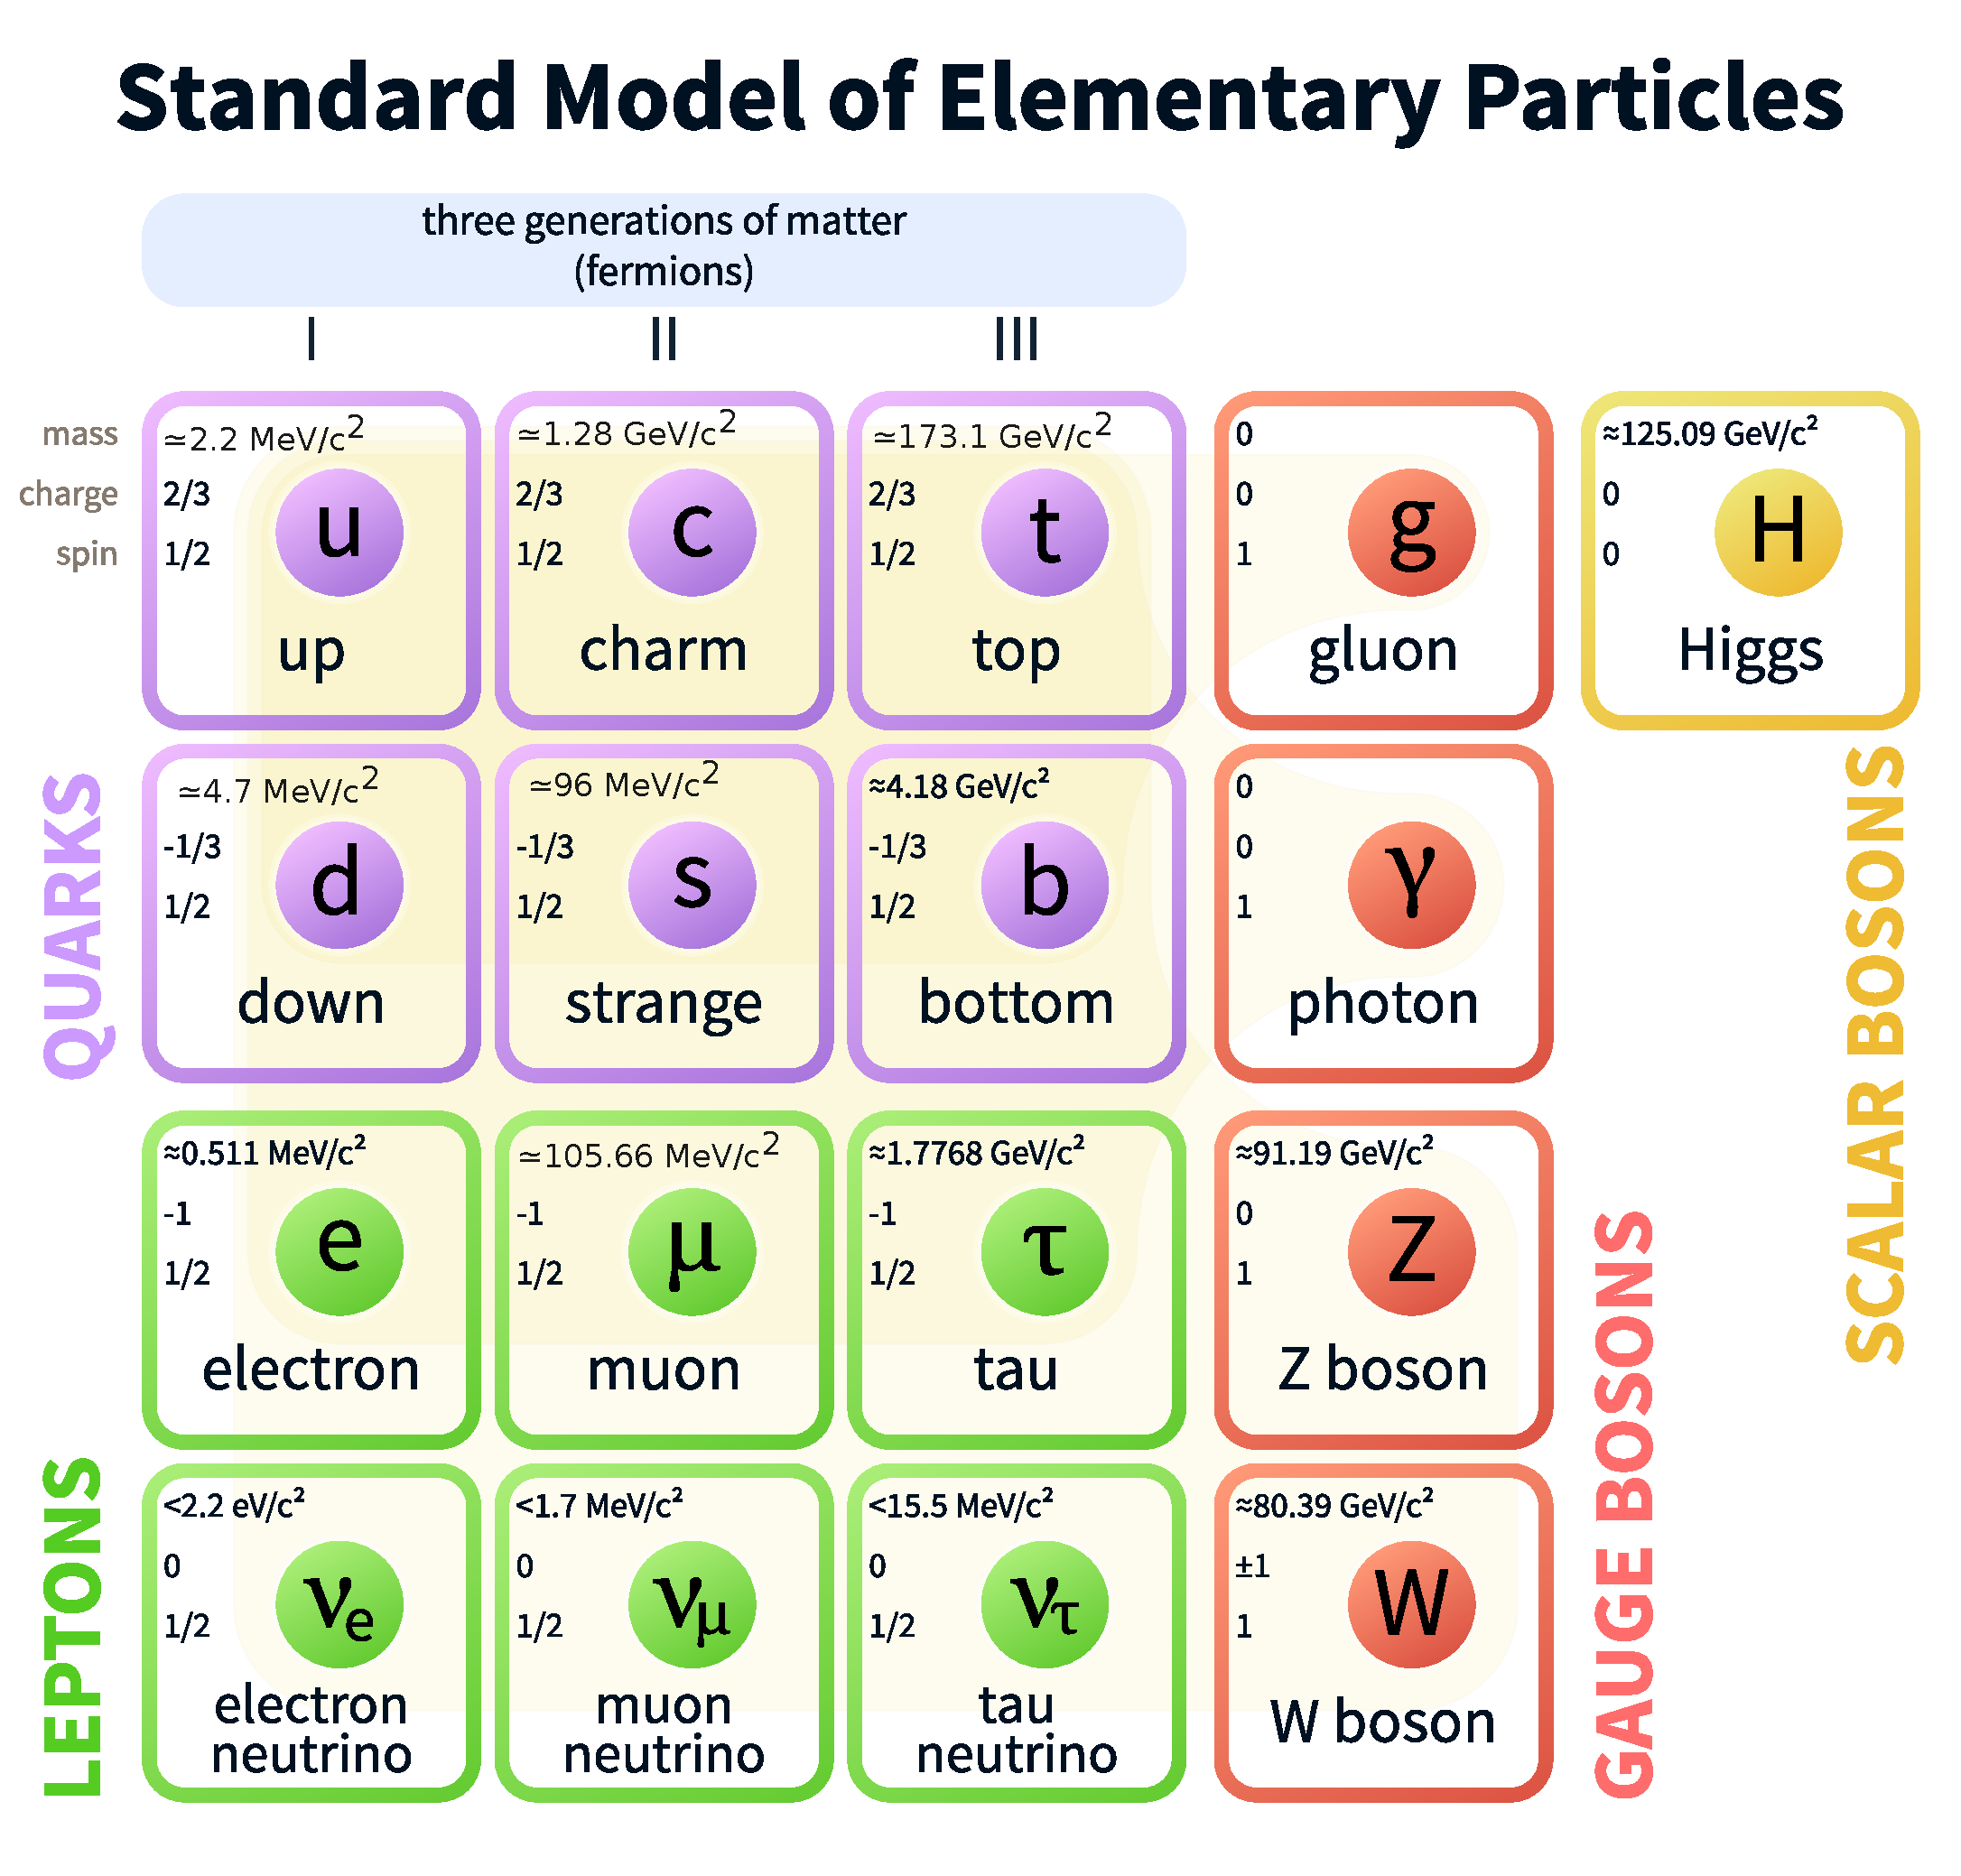
\includegraphics[width=0.6\textwidth]{figs/StandardModelofElementaryParticles.pdf}
\caption{The particles of the Standard Model.}
\label{fig:sm}
\end{figure}

\section{Quantum Electrodynamics}

Quantum electrodynamics describes the interactions of particles with electric charge. The interactions arise naturally by requiring the free-particle Dirac Lagrangian to be invariant under the U(1) transformation:

\begin{equation}
\psi(x)  \xrightarrow[]{\text{U(1)}} e^{i q \alpha(x)}\,\psi(x)
\label{eq:u1}
\end{equation}
where $q$ is the electric charge, and $\alpha$ is an arbitrary function of spacetime. $\psi$ is a single Dirac fermion.

U(1) gauge-invariance requires us to modify the definition of the partial derivative to include a spin-1 vector field $\mathrm{A}_{\mu}$, the photon:
\begin{equation}
\begin{array}{l}
\partial{\mu} \rightarrow\ \partial_{\mu} - iq\mathrm{A}_{\mu}
\\A_{\mu} \xrightarrow[]{\text{U(1)}} \mathrm{A}_{\mu} - q \partial_{\mu} \alpha
 \end{array}
\end{equation}

The complete Lagrangian becomes:
\begin{equation}
\mathcal{L}_{\mathrm{QED}} =
i\bar{\psi}\gamma^{\mu}\partial_{\mu}\psi
- q\bar{\psi}\gamma^{\mu}\psi \mathrm{A}_{\mu}
- m\bar{\psi}\psi
- \frac{1}{4}\mathrm{F}_{\mu\nu} \mathrm{F}^{\mu\nu}
\end{equation}

where $\mathrm{F}_{\mu\nu}\equiv\partial_{\mu}\mathrm{A}_{\nu} - \partial_{\nu}\mathrm{A}_{\mu}$, is known as the \textit{field strength tensor} and represents the kinetic energy of the photon field. A photon mass term $\frac{1}{2}m^{2}\mathrm{A}^{\mu}\mathrm{A}_{\mu}$ is forbidden as it is not invariant under the transformation rule.

\section{Quantum Chromodynamics} 

Quantum chromodynamics describes the strong force - interactions of particles with color charge. The interactions arise naturally by requiring the free-particle Dirac Lagrangian to be invariant under the SU(3) transformation:

\begin{equation}
\psi(x) \xrightarrow[]{\text{SU(3)}} e^{\frac{1}{2}ig_{s}\bm{\alpha(x)}\cdot\bm{\lambda}}\,\psi(x)
\end{equation}
where $g_{s}$ is the strong coupling constant, $\bm{\alpha}$ is an arbitrary 8-dimensional vector of spacetime, and $\bm{\lambda}$ are the 8 3x3 Gell-Mann matrices. $\psi$ is a color triplet of Dirac fermions $\bar{\psi} = (\psi_{red}, \psi_{blue}, \psi_{green})$.

SU(3) gauge invariance requires us to modify the definition of the partial derivative to include 8 spin-1 vector fields $\bm{G}_{\mu}$, the gluons:
\begin{equation}
\begin{array}{l}
\partial{\mu} \rightarrow \partial_{\mu} - i g_{s} \bm{\lambda} \cdot \bm{G}_{\mu}\\
G^{k}_{\mu} \xrightarrow[]{\text{SU(3)}} G^{k}_{\mu} - g_{s}\partial_{\mu}\alpha_{k} - g_{s}f_{ijk}\alpha_{i}G^{j}_{\mu}
\end{array}
\end{equation}
where $f_{ijk}$ are known as the \textit{structure constants} of SU(3) and arise from its non-abelian nature, they satisfy $[\lambda_{i},\lambda_{j}] = 2if_{ijk}\lambda_{k}$. This term is responsible for the self-coupling within the gluon field.

The complete Lagrangian becomes:
\begin{equation}
\mathcal{L}_{\mathrm{QCD}} =
i \bar{\psi} \gamma^{\mu} \partial_{\mu} \psi
- (g_{s} \bar{\psi} \gamma^{\mu} \bm{\lambda} \psi) \cdot \textbf{G}_{\mu}
- m \bar{\psi} \psi
- \frac{1}{16\pi} \textbf{G}^{\mu\nu} \cdot \textbf{G}_{\mu\nu}
\end{equation}

where $G^{\mu\nu}_{i} \equiv \partial^{\mu} G^{\nu}_{i} - \partial_{\nu} G^{\mu}_{i} - 2 q f_{ijk} G^{\mu}_{j} G^{\nu}_{k}$ is the field strength tensor for the gluon fields.

The presence of theThe gluon mass term $\frac{1}{2}m^{2}\bm{\mathrm{G}}^{\mu} \cdot \bm{\mathrm{G}}_{\mu}$ is forbidden as it is not invariant under the transformation rule and they remain massless.

\section{Electroweak Theory}

Electroweak theory is a quantum field theory which provides a description of the weak nuclear force between particles with \textit{weak isospin} and \textit{hypercharge} quantum numbers. In concert with this description comes that of electrodynamics, thereby uniting the two in a single framework. The theory is generated by demanding local invariance of the Lagrangian under a combined SU(2)$\times$U(1) symmetry. Four new gauge fields must be introduced into the theory to give the proper transformation rule of the covariant derivate. Mixing between these fields generates the physical W$^{\pm}$ boson, Z boson, and photon. Under SU(2)$\times$U(1), the fields transform in the following manner:

\begin{equation}
\begin{array}{l}
\psi(x) \xrightarrow[]{\text{U(1)}} e^{i g' \frac{Y}{2} \alpha(x)} \, \psi(x) \\
\psi_{L}(x) \xrightarrow[]{\text{SU(2)}} e^{i g_{W} \bm{\xi}(x) \cdot \frac{1}{2} \bm{\sigma} } \, \psi_{L}(x) 
\end{array}
\end{equation}
where $g'$ is the hypercharge coupling constant, Y is the hypercharge operator, $g_{W}$ is the weak coupling constant, $\alpha$ and $\xi$ are arbitrary functions of spacetime, and $\bm{\sigma}$ represents the 3 2x2 Pauli spin matrices. $\psi_{L}$ is an \textbf{isospin doublet} made of the following fermion anti-fermion pairs:

\begin{equation*}
\begin{pmatrix} \nu_{e} \\ e \end{pmatrix},
\begin{pmatrix} \nu_{\mu} \\ \mu \end{pmatrix},
\begin{pmatrix} \nu_{\tau} \\ \tau \end{pmatrix},
\begin{pmatrix} u \\ d' \end{pmatrix},
\begin{pmatrix} c \\ s' \end{pmatrix},
\begin{pmatrix} t \\ b' \end{pmatrix}
\end{equation*}

The weak force is a \textit{chiral} theory which does not treat the left and right-chiral components of a Dirac fermion equally.  The projection operator $P_{R,L} = \frac{1}{2} ( 1 \pm \gamma^{5})$ defines these states and all fermions can be decomposed as $\psi = \psi_{L} + \psi_{R}$. Within the electroweak theory, isospin doublets consist of pairs of left-chiral particles and right-chiral antiparticles.

As usual, SU(2) and U(1) gauge-invariance requires us to modify the definition of the partial derivate to include three spin-1 vector fields $\bm{\mathrm{W}}^{\mu}$ and a single spin-1 vector field B$^{\mu}$:

\begin{equation}
\begin{array}{l}
\partial{\mu} \rightarrow\ \partial_{\mu} - i g' \frac{Y}{2}\mathrm{B}_{\mu} -  i g_{W} \frac{1}{2}\bm{\sigma} \cdot \bm{\mathrm{W}}_{\mu}\\
\mathrm{B}_{\mu} \xrightarrow[]{\text{U(1)}} \mathrm{B}_{\mu} - i g' \partial_{\mu} \alpha \\
\mathrm{W}^{k}_{\mu} \xrightarrow[]{\text{SU(2)}} W^{k}_{\mu} - g_{W} \partial_{\mu} \alpha^{k} -  g_{W} \epsilon_{ijk} \xi^{i} W^{j}_{\mu}
 \end{array}
\end{equation}
where $\epsilon_{ijk}$ is the totally antisymmetric Levi-Civita tensor (the structure constants of SU(2)).

Because of the SU(2) symmetry, we must introduce \textbf{two} Dirac fermions to the theory, where the left and right chiral components are treated differently. Without loss of generality we will label these fields at $\bar{\psi} = (\chi \, \xi)$, but these can be any of the available pairs listed above. The Lagrangian will be written in terms of these new fields:

The complete Lagrangian becomes:
\begin{equation}
\begin{array}{l}
\mathcal{L}_{\mathrm{EWK}} = 
i \bar{\chi} \gamma^{\mu} \partial_{\mu} \chi - m \bar{\chi} \chi
+ i \bar{\xi}   \gamma^{\mu}    \partial_{\mu} \xi  - m \bar{\xi} \xi
- \frac{1}{4}\mathrm{}B_{\mu\nu}\mathrm{B}^{\mu\nu}
-\frac{1}{4}\bm{\mathrm{W}}_{\mu\nu} \cdot \bm{\mathrm{W}}^{\mu\nu} \\
\hspace{1.2cm}
-  g' \bar{\chi} \gamma^{\mu} \frac{Y}{2} \chi B_{\mu} + g' \bar{\xi} \gamma^{\mu} \frac{Y}{2} \xi B_{\mu}
- g_W  \bar{\psi} \gamma^{\mu} \bm{\sigma} \psi \cdot \bm{\mathrm{W}}_{\mu}
\end{array}
\end{equation}

The B$^{\mu}$ and $\bm{\mathrm{W}}^{\mu}$ bosons remain massless as mass terms would not be invariant under the symmetry transformation rule for the vector fields. The observable W and Z bosons are indeed massive, so mass terms must be generated through some other mechanism.

\subsection{The Higgs Mechanism}

As has been mentioned, the gauge bosons in the electroweak theory must remain massless as the appropriate term in the Lagrangian would not remain invariant under the transformation rule of the field. Additionally, it has not been mentioned that the fermion mass terms $-m\bar{\psi}\psi = -m( \bar{\psi}_{R} \psi_{L} + \bar{\psi}_{L}\psi_{R})$ are forbidden as they are not invariant under the chiral-transformation of the theory treating the left and right-chiral components differently. The Higgs mechanism is able to generate mass terms for the W, Z, and fermions within the Standard Model. This is an essential component and its discovery in 2012 was monumental. \cite{higgsdisc}

This Higgs mechanism proceeds by introducing a massive spin-0 complex scalar field with the following Lagrangian.
\begin{equation}
\mathcal{L} = \frac{1}{2} (\partial_{\mu}\phi^{\dagger})(\partial^{\mu}\phi) - \frac{1}{2}\mu^{2} \phi^{\dagger}\phi + \lambda(\phi^{\dagger}\phi)^{2}
\end{equation}
where $\mu$ and $\lambda$ are the strengths of the self-coupling terms.

The field in the Standard Model is in fact an isospin doublet consisting of electrically neutral and charged components:
\begin{equation}
\phi = \begin{pmatrix} \phi^{+} \\ \phi^{0} \end{pmatrix} = \begin{pmatrix} \phi_{1} + i\phi_{2} \\  \phi_{3} + i\phi_{4} \end{pmatrix},
\end{equation}

Solving for the minimum of the potential, it is found that the ground state of $\phi$ is non-zero and satisfies $\phi^{\dagger}\phi = \phi_{1}^{2} + \phi_{2}^{2} + \phi_{3}^{2}  + \phi_{4}^{2} = \frac{v^{2}}{2} = - \frac{\mu^{2}}{2\lambda}$. As particles are represented as fluctuations above the vacuum, we must express the fields in the same manner. Electric charge conservation requires that this \textit{vacuum expectation value} lie entirely inside the neutral $\phi^{0}$ which is rewritten as $\phi^{0} = v + h(x)$, where $h(x)$ is to be identified as the Higgs boson.

\subsubsection{Masses of the W and Z bosons}

The kinetic energy term $\frac{1}{2} (\partial_{\mu}\phi^{\dagger})(\partial^{\mu}\phi)$ for the Higgs boson introduces a coupling with the $\bm{\mathrm{W}}^{\mu}$ and B$^{\mu}$ bosons when they are added to the covariant derivate:

\begin{equation}
\partial_{\mu}\phi = (\frac{1}{2}\partial_{\mu} + \frac{1}{2} i g_{W}\bm{\sigma}\cdot\bm{\mathrm{W}} + i g' \frac{Y}{2} B^{\mu})\begin{pmatrix} 0 \\ v + h(x) \end{pmatrix}
\end{equation}

After performing the matrix calculations, and lots of algebra, we see there are terms quadratic in the gauge fields:
\begin{equation}
\frac{1}{8} v^{2} g_{W}^{2} ( W^{1}_{\mu} W_{1}^{\mu} + W^{2}_{\mu} W_{2}^{\mu}) + \frac{1}{8} v^{2} ( g_{W} W^{3}_{\mu} - g'B_{\mu} ) ( g_{W} W_{3}^{\mu} -g' B^{\mu} )
\end{equation}

Where we see we have generated mass terms for the W$^{\mu}_{1,2}$ fields: $\frac{1}{2} v^{2} g_{W}^{2} W^{\mu}W_{\mu}$. The last term in the expansion introduces mixed couplings between the W$_{3}^{\mu}$ and B$^{\mu}$ fields and the term can be represented as a mass matrix with non-diagonal entries - physical particles are eigen states of the mass matrix. Upon diagonalization, we find the states corresponding to the physical particles:

\begin{equation}
\begin{array}{l}
A_{\mu} = \frac{1}{\sqrt{g_{W}^{2} + g'^{2}}} \, (g' W^{3}_{\mu} + g_{W}B_{\mu});\hspace{0.5cm} \mathrm{with\,\,mass}\,\,0\\
Z_{\mu} = \frac{1}{\sqrt{g_{W}^{2} + g'^{2}}} \, (g_{W} W^{3}_{\mu} - g'B_{\mu}); \hspace{0.5cm} \mathrm{with\,\,mass}\,\, \frac{1}{2}v\sqrt{g_{W}^{2} + g'^{2}}
\end{array}
\end{equation}
where $A_{\mu}$ corresponds to the photon of electromagnetism, and $Z_{\mu}$ the neutral gauge boson responsible for the weak neutral currents.

The physical W bosons are in fact linear combinations of the $\mathrm{\bm{W}}^{\mu}$ fields: $W^{\pm}_{\mu}= \frac{1}{\sqrt{2}}(\mathrm{W}^{1}_{\mu} + \mathrm{W}^{2}_{\mu})$. These correspond to the raising and lowering operators of SU(2) and therefore step between states with differing isospin component $I_{3}$, indicated in the doublet pairings seen above.

We have seen how the Higgs mechanism is able to generate mass terms for the gauge bosons in the electroweak theory.

\subsubsection{Masses of the Fermions}

Up to this point, it has not been mentioned that the fermion mass term $m\psi\bar{\psi}$ is not invariant under the SU(2) symmetry - the left-chiral states transform as isospin doublets whereas the right-chiral states transform as singlets. This is made explicit by using the projection operators to decompose a Dirac fermion into left and right chiral components $-m\bar{\psi}\psi = -m(\bar{\psi}_{L}\psi_{R} + m\bar{\psi}_{R}\psi_{L})$. As the fermion masses are all non-zero, some mechanism must be built into the Standard Model to generate mass terms. This is done by introducing an interaction between the Higgs field and fermions. Consider the following Lagrangian:

\begin{equation}
\mathcal{L} = -y ( \bar{\psi_{L}} \phi \psi_{R} + \bar{\psi_{R}} \phi^{\dagger} \psi_{L})
\end{equation}
where $y$ is the \textit{Yukawa coupling}, $\bar{\psi_{L}}$ is an isospin doublet of left-chiral fermions, and $\psi_{R}$ is a right-chiral fermion.

\section{Parameters of the Standard Model}

Throughout this chapter we have encountered 15 parameters that must be specified as an input to the theory which must all be determined experimentally. Here is the list:
\begin{itemize}
\item the 9 quark and lepton masses: $m_{u}, m_{d}, m_{s}, m_{c}, m_{b}, m_{t}, m_{e}, m_{\mu}, m_{\tau}$
\item 4 CKM matrix elements, often parametrized by $\lambda, A, \rho, \eta$
\item the Higgs mass and quartic coupling: $m_{H}, \lambda$
\end{itemize}

Inclusion of massive neutrinos in the theory creates an additional 7 parameters:
\begin{itemize}
\item three neutrino mass eigenstates: $m_{\nu_{1}}, m_{\nu_{2}}, m_{\nu_{3}}$
\item four parameters for the PMNS matrix, governing mixing between the neutrino mass and flavor states (analogous to the CKM matrix).
\end{itemize}
Although the exact implementation of their masses in the SM is unknown.
